\chapter{Method}
\label{sec:method}



\section{Overview}

\begin{figure}[h]
    \centering
    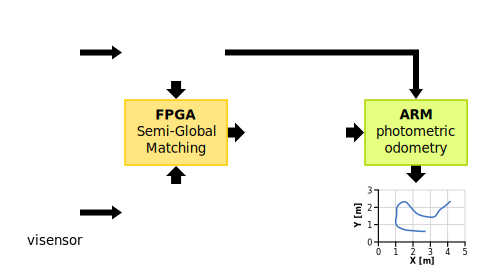
\includegraphics[width=\textwidth]{images/system_overview.pdf}
    \caption{schematic overview of the whole system}
    \label{fig:overview}
\end{figure}


The visensor provides a stream of frames, each of which consists of a stereo
pair of intensity data \footnote{Grayscale instead of full-color images are
used, because the information gain from colors is offset by the loss of
resolution. However, the approach described here would work similarly colors.}.

A semiglobal stereo matching core developed by [todo: ref] running on the FPGA
processes these and produces a disparity image which assigns every pixel the
disparity between the two cameras. The FPGA also provides a rectified camera
image.

This pair of intensity and disparity images is conceptually equivalent to a
three dimensional point-cloud, as we can calculate the distance to the camera
for every pixel from the disparity data. This is in turn makes it possible to
render the point-cloud from an arbitrary perspective, allowing us to look at an
image as if it was recorded from a different angle.

To estimate the ego-motion between two frames we can thus look for a
perspective that looks the same as the previous frame.  The movement of the
virtual camera will then correspond to the actual, physical movement of the
sensor.

By subtracting the intensities from the previous frame with the
intensities of the current frame sampled at the warped pixel locations a
photometric error is calculated, measuring the similarity of the warped current
frame with the previous one. The problem is now to minimize this error function.

Note that this approach assumes photoconsistency: Points have the same
intensity, regardless of viewing angle.


\section{Warping Pipeline}

\begin{figure}[h]
    \centering
    \includegraphics[width=\textwidth]{images/warp_pipeline.pdf}
    \caption{the full warping pipeline (pink pixels are not sampled by any of the warped points)}
    \label{fig:warp_pipeline}
\end{figure}

This section closely follows \cite{omaridenseodometry}.

Using an inverse projection derived from the standard pinhole camera model, a
point $ \vec{x} $ in the camera image plane can be back-projected into a point
$ \vec{p} $ in $ \mathbb{R}^3 $:

\begin{equation}
    \label{eq:backprojection}
    \vec{p} = \pi^{-1}(\vec{x}, D(\vec{x})) := \frac{b}{D(x)}
    \begin{bmatrix}
        \vec{x_u} - \vec{c_u} \\
        \vec{x_v} - \vec{c_v} \\
        f
    \end{bmatrix}
\end{equation}

where $b$ is the stereo baseline, $f$ the focal length and $\vec{c}$ the principal point of the camera.

This point $\vec{p}$ can now be moved into a new camera frame by translating and rotating it:

\begin{equation}
    \vec{p'} = \mat{T_R} \cdot \vec{p} + \vec{T_T}
\end{equation}

Where $T_R$ is a 3x3 rotation matrix and $T_T$ a three dimensional translation
vector. Using affine coordinates, we can write this as:

\begin{equation}
    \vec{p'} = \mat{T} \vec{p}
\end{equation}

A point in 3D space can be projected back onto the (now moved) camera image plane:

\begin{equation}
    \label{eq:projection}
    \vec{x'} = \pi(\vec{p'}) := \frac{f}{\vec{p'}_z}
    \begin{bmatrix}
        \vec{p'}_x \\
        \vec{p'}_y \\
    \end{bmatrix}
    + \vec{c}
\end{equation}

This whole warping operator can be summarized in a warping operator $\tau$:

\begin{equation}
    \vec{x'} = \tau(\vec{x}, D(\vec{x}), \vec{T}) := \pi( \mat{T} \cdot \pi^{-1} (\vec{x}, D(\vec{x})))
\end{equation}



\section{Minimization}

Using $\tau$, the error between the previous frame and the warped current frame can be defined as:

\begin{equation}
    e(\vec{x}, \vec{T}) := I_p(\tau(\vec{x}, \vec{T})) - I_c(\vec{x})
\end{equation}


To estimate the motion between two frames, this photometric error term should
be minimal for every pixel:

\begin{equation}
    \vec{\hat{T}} = \operatornamewithlimits{argmin}_{\vec{T}} \sum_{\vec{x} \in I_p} e(\vec{x}, \vec{T})^2
\end{equation}


This equation can be solved for the estimated motion by applying standard
optimization techniques, for exmple Gauss-Newton:

\begin{equation}
    \mat{J}^T \mat{J} \Delta \vec{T} = - \mat{J}^T \vec{e(\vec{T})}
\end{equation}

Here, $\mat{J} \in \mathbb{R}^{N \times 6}$ is the stacked Jacobian matrices
and $\vec{e(\vec{T})} \in \mathbb{R}^N$ the vector of the error terms of all
$N$ pixels.  This equation is iteratively solved for the increment $\Delta
\vec{T}$ of the motion estimation after recalculating the error term and
Jacobians from the new estimation.

The Jacobian is derived by applying the chain rule to photometric error term.
For a single pixel, we get a $1 \times 6$ Jacobian:

\begin{equation}
    \mat{J} := \mat{J_I} \mat{J_{\pi}} \mat{J_T}
\end{equation}

where $\mat{J_I} \in \mathbb{R}^{1 \times 2}$ is the image derivative of the warped previous frame and is
approximated using the image's gradient:

\begin{equation}
    \mat{J_I} := \frac{\partial \mathbf{I_p}(\vec{x})} {\partial \vec{x}} \bigg|_{\vec{x} = \tau(\vec{x}, \vec{T})}
    \approx
    \begin{bmatrix}
        \nabla{}_x \mathbf{I_p} & \nabla{}_y \mathbf{I_p}
    \end{bmatrix}
\end{equation}

The term $\mat{J_{\pi}}$ is the $2 \times 3$ Jacobian of the projection
function \ref{eq:projection}, evaluated at the warped 3D point:

\begin{equation}
    \mat{J_{\pi}} := \frac{\partial \pi(\vec{p})}{\partial \vec{p}}
    \bigg|_{\vec{p} = \vec{T}\cdot\pi^{-1}(\vec{x},\mathbf{D}(\vec{x}))}
    =
    \begin{bmatrix}
        \nicefrac{f}{\vec{p_z}} & 0 & -f \nicefrac{\vec{p_x}}{\vec{p_z}^2} \\
        0 & \nicefrac{f}{\vec{p_z}} & -f \nicefrac{\vec{p_y}}{\vec{p_z}^2}
    \end{bmatrix}
\end{equation}

$\mat{J_T}$ is the $3 \times 6$ Jacobian of the transformation operator $T$ and
the most costly term to compute:

\begin{equation}
    \mat{J_T} := \frac{\partial (\vec{T} \vec{p})}{\partial \vec{T}}
    \bigg|_{\vec{p} = \pi^{-1}(\vec{x}, \mathbf{D}(\vec{x}))}
\end{equation}








\section{Optimizations and other improvements}
\label{sec:optimizations}

The algorithm described in the previous section works well but suffers from
slow performance and does not nearly run in realtime on an embedded device.
Therefore, some optimization strategies are applied:

\subsection{Image pyramids}
\label{sec:pyramids}

A common optimization technique is the use of multiple resolutions: Images are
repeatedly downscaled by a factor of two (essentially quartering the number of
pixels) by averaging over a 2 x 2 block to generate a stack of increasingly
smaller images (a 'pyramid').

The minimization is run on the smallest set of images and the resulting value
is used as an initial value for the next bigger set of images.

This greatly reduces the number of iterations required and enhances the
convergence radius.

The image pyramid can also be used to trade a bit of accuracy for even more
performance gain by simply aborting early and not using the full resolution at
all. Throwing out the one or two uppermost levels usually incurs negligible
loss of accuracy. See also section~\ref{sec:results_qualitative}.


\subsection{Pixel selection by image gradient}
\label{subsec:gradient_filtering}

We can further optimize away pixels which do not strongly influence the
minimization such as points in homogenous image regions where $\nabla
\mathbf{I} \approx 0$ and therefore $\mat{J_I} \approx 0$.

This is already provided to some extent by the semi-global matching alorithm,
as pixels without strong gradients are usally hard to match and therefore often
don't provide a disparity value.

\subsection{Handling outliers}

By robustly weighting the photometric error terms outliers can be dampened to
reduce the influence of occlusions, moving scenery or other noise, such as
errors from the semi-global matcher. This improves quality and stability with
negligible performance penalty.

Another idea (which wasn't fully investigated) to handle occlusions is to use a
Z-buffer to eliminate points which are behind others when warped.


\subsection{Further possible optmiziations}

A few things which have not been investigated in this work but which provide
good avenues for further optimizations:

\subsubsection{integration of IMU}

Modern visual odometry and SLAM systems such as \cite{leutenegger2013keyframe}
incorporate data from an inertial measurement unit using various complicated
filtering schemes to increase accuracy.

In contrast, using integrated acceleration values for pohotometric odometry
would be trivial by providing a good initial guess for the minimization process
and could greatly speed up perfomance by reducing the number of required
optimization iterations.

\subsubsection{Keyframes}

Instead of matching the previous frame, keyframes can be used which are only
updated when the relative motion gets too big. This way, drift can be reduced
and even completely eliminated when being more or less stationary.

\subsubsection{Offload more work to FPGA}

Large parts of the photometric odometry algorithm are highly parallelizable and
would profit from an implementation running on the FPGA. This is the main point
of this work and is further discussed in section~\ref{sec:timing}.



\section{Implementation details}

A few things that are only tangentially related to the core algorithm but which
nevertheless might be encountered in an actual implementation:

\subsection{Representation of transformation}

A six degree of freedom transformation can be represented in multiple ways.
While translations are very straightforward, rotations can be represented in
numerous ways (Euler-angles, quaternions, rotation matrices, etc.) and proper
derivation of the Jacobians can be tricky.

Fortunately, odometry works in a relative fashion without any absolute
orientation and steps are very incremental as photometric odometry cannot
handle more than a few degrees of rotation. This implies we do not have to deal
with gimbal-lock and other mathematical hurdles of working in $SO(3)$.

\subsection{Image scaling}

Care has to be taken to properly downscale image coordinates when working with
image pyramids. This can be done by scaling the camera intrinsics properly:
Halving the image width also means halving the focal length and doubling the
baseline.

Downscaling usually implies filtering and doing so alters the 3D structure. For
this reason, [ref to comport ICP] does not downscale the disparity values and
samples them at the full resolution. When matching pose on the camera plane
instead of in 3D space, downscaling the disparity values works as well
\footnote{It might be worth investigating how much of an effect on performance
and quality downscaling the disparity images has. Disparity values are only
read at integer coordinates and downscaling them might not be worth the runtime
penalty.}.

\subsection{Ignore invalid pixels}

Pixels that do not have a disparity value (because the SGM algorithm couldn't
find any correspondence) can obviously be ignored. So can pixels which are
saturated or underexposed: They do not provide valid disparity data and are
often not photoconsistent either.

\subsection{Don't remove too many pixels}

The optimizations described in section~\ref{sec:optimizations} can
substantially reduce the pixel count, so much so that there are not enough for
stable performance. Especially filtering pixels based on their image gradient
as explained in section~\ref{subsec:gradient_filtering} requires a well-chosen
threshold, as image gradients depend on the scene. [ref to ICP] proposes the
calculation of a histogram to select the $N$ best pixels. An easier approach is
to simply restart the current iteration with a lower threshold when the number
of pixels gets too low and increasing it after a step with enough pixels. The
same problem also applies to other optimization parameters such as the size of
the image pyramid.
